\chapter{Les plaques résistives de verre de basse résistivité}
\renewcommand\chapterillustration{GLA/gla}
\ThisULCornerWallPaper{1}{\chapterillustration}
\minitoc

\lettrine[lines=4, slope=-0.5em]{C}{e} chapitre comporte une description des plaques résistives de verre de basse résisitivité ainsi que certaines de leur caractéristiques. Il comporte également les résultats obtenus lors des nombreuses campagnes de tests en faisceaux organisé au SPS, PS et Gamma Iradiation Facility (GIF++). Ces résultats ont fait l'objet d'une conférence lors de RPC2016 à ghent, de plusieurs proceeding \cite{Lagarde:2016fvf}\cite{Gouzevitch:2016pcr} ainsi que de nombreux posters.


\section{Le verre dopé de base résistivité}
Une des solution pour augmenter la capacité de détection des RPC est d'utilisé du verre de basse résistivité comme électrodes. Le nouveau verre dopé, développé par l'université de Tsinghua (Chine) présente une résitivité de l'ordre de $10^10ohms.cm$ et une très bonne uniformité de surface. Ce type de verre sera utilisé dans l'expérience \textit{Compressed Baryonic Matter} (CBM) \cite{Wang:2016bsx}. Certaines caractéristiques de ce verres sont répertorié dans le tableau \ref{tabb}
\begin{table}[H]
	\centering
	\begin{tabular}{|O|O|N}
	\hline 
	Dimenssion maximale  &32cm$\times$30cm \\ 
	\hline 
	Résistivité volumique & $10^10 ohm.cm$ \\ 
	\hline 
	Épaisseur & 0.5mm-2mm \\ 
	\hline 
	Uniformité de l'épaisseur & 0.02mm \\
	\hline
	Constante diélectrique & 7.5-9.5  \\ 
	\hline 
	Rugosité & $<10nm$ \\ 
	\hline
\end{tabular} 
\captionof{table}{Caractéristique du verre dopé.}
\label{tabb}
\end{table}
La résistivité de ces verre est 100 à 1000 fois moins importante que celle de verre standard (float glass), ce qui rend ce verre très intéressant pour la détection de particule à haut flux. La résistivité de ce matériaux se révèle également très stable même après une charge intégré de $1C/cm^2$ (cf.fig\ref{resi})
\begin{figure}[h!]
	\centering
	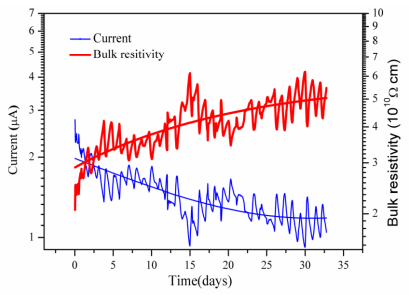
\includegraphics[width=1\textwidth]{GLA/resi.png}
	\captionof{figure}{Évolution du courant (courbe bleue) et de la résistivité volumique (courbe rouge) en fonction du temps d'une électrode de verre de basse résistivité soumise à une tension de 1000V pendant 32 jours.}
	\label{resi}
\end{figure}
La rugosité est excellente ce qui permet de n'appliquer aucun traitement de surface; contrairement au RPC en bakélite. Ces traitements se sont révélés problèmatique au cours des années.

L'inconvénient majeur de ce matériaux est sa dimension maximale qui ne peut excéder 32cm*30cm (cf.fig\ref{verre}). En effet de par le procéder de fabrication (cf.fig\ref{cooling}) de ces verres et par leur pollisage à la main, de plus grandes dimensions sont irréalisables.
\marginpar
{
	\centering
	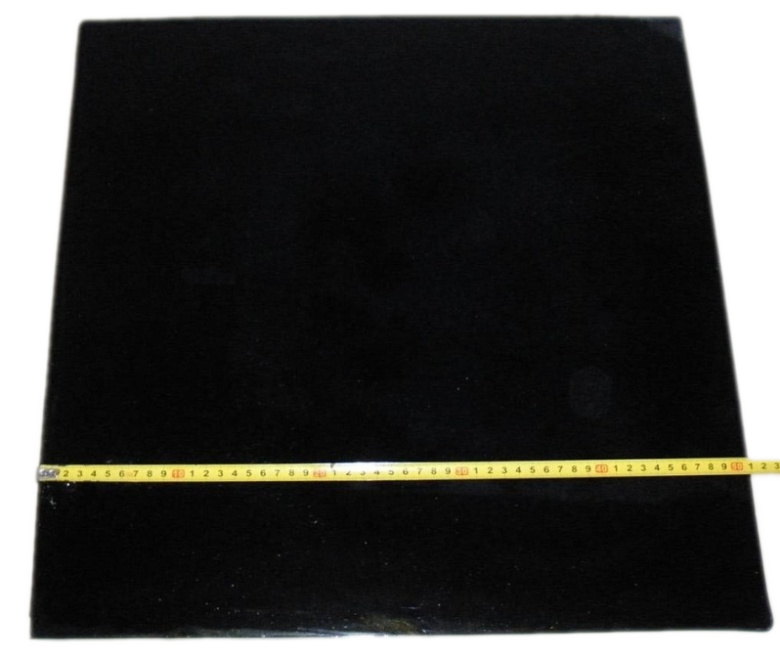
\includegraphics[width=\marginparwidth]{GLA/verre.png}
	\captionof{figure}{Photo d'une électrode de verre de basse résistivité.}
	\label{verre}
}
\marginpar
{
	\centering
	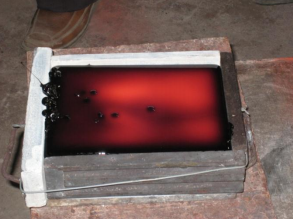
\includegraphics[width=\marginparwidth]{GLA/cooling.png}
	\captionof{figure}{Refroidissement d'un bloc de verre de basse résistivité.}
	\label{cooling}
}

Des détecteurs de cette dimension ont donc été construit afin d'étudier leur caractéristiques et de voir s'ils étaient compatibles avec les demandes de CMS.

\section{Caractérisation des Glass Resitive Plate Chamber (GRPC)}
 
L'étude des GRPC passe par la connaissance de trois caractéristique principales :
\begin{itemize}[label=$\bullet$]
	\item \textbf{L'Efficacité} de détection des particules. C'est la caractéristiques principales. Elle est calculée en faisant le rapport entre le nombre de particules ayant été détectées et le nombres de particules ayant traversée le détecteur. Bien sûr, dans le cas où le signal est récolté par une électronique à seuil, la valeur de celui-ci va affecter l'efficacité de détection.
	\item \textbf{La multiplicité} représente le nombres de cellules ou bandes touchés lorsqu'une particule traverse le détecteur. En effet, plusieurs cellules de détections peuvent être déclenchées par le courant induit par les électrons créés lors de l'avalanche. Ici aussi le seuil appliqué à l'électronique influe sur la valeur de la multiplicité. La multiplicité joue un rôle très important sur la résolution spatiale du détecteur comme on le verra par la suite.
	\item \textbf{Le bruit électronique} qui est la fréquence de détection par l'électronique, d'un signal considéré comme non physique. Ceci peut être dû à une avalanche d'origine thermique ou radiative, par un courant dans le couche résistive etc. 
\end{itemize}

Un bon détecteur doit donc être proche d'une efficacité de 100\% avec une fréquence de bruit très basse. La multiplicité idéale dépend de la taille des cellules, du seuil appliqué et surtout de la résolution spatiale que l'on veut atteindre. D'autres caractèristiques du détecteurs sont imporatntes telles que la sensibilité au bruit de fond (photon et neutrons par exemple) et l'évolution des caractéristiques du détecteurs en fonction du temps, ce que l'on appelle le vieillissement du détecteurs.

Ces détecteurs ont été instrumenté avec une électronique dite semi-digitale utilisé depuis de nombreuses années aux laboratoire dans un prototype de calorimètre hadronique semi digitale (SDHCAL) (cf.fig\ref{SDHCAL}) \cite{Buridon:2016ill} pour le détecteur International Large Detector (ILD) (cf.fig\ref{ILD}); L'un des deux détecteurs de l'expérience International Linear Collider (ILC) (cf.fig\ref{ILC}).
\marginpar
{
	\centering
	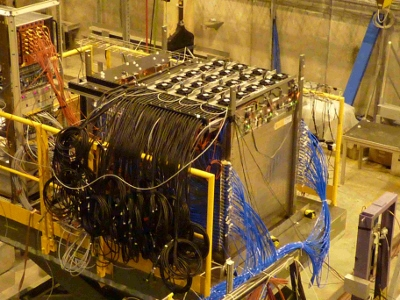
\includegraphics[width=\marginparwidth]{GLA/SDHCAL.jpg}
	\captionof{figure}{Photo du prototype SDHCAL construit à Lyon.}
	\label{SDHCAL}
}
\marginpar
{
	\centering
	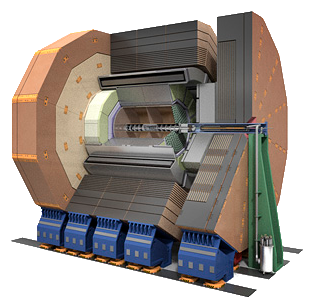
\includegraphics[width=\marginparwidth]{GLA/ILD.png}
	\captionof{figure}{Schéma de l'ILD.}
	\label{ILD}
}
\marginpar
{
	\centering
	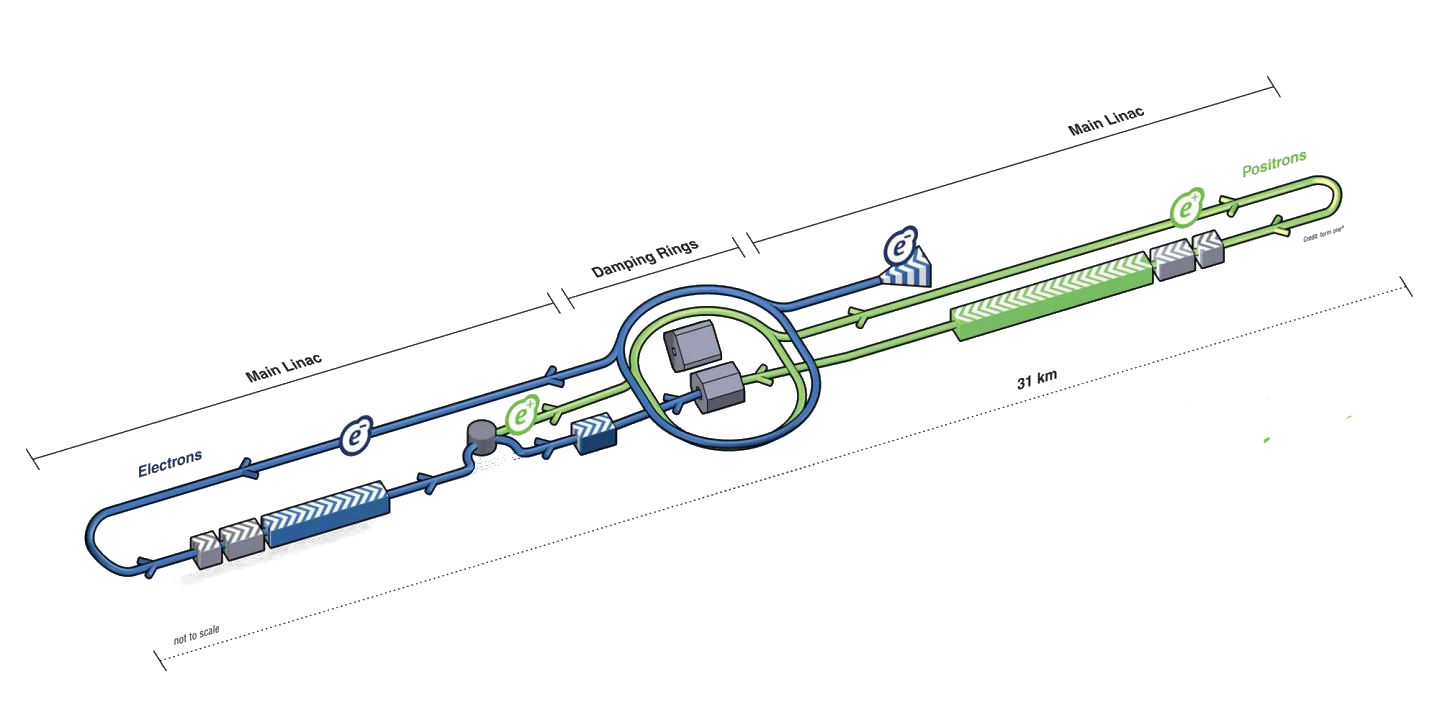
\includegraphics[width=\marginparwidth]{GLA/ILC.png}
	\captionof{figure}{Schéma de l'accélérateur ILC.}
	\label{ILC}
}

\section{Électronique "semi-digitale"}
Le calorimètre SDHCAL a nécessité la création d'un système électronique digital à plusieurs seuils, ceci afin de réduire à la fois l'énergie thermique dissipée et la quantité de donnée. La conversion en signal digital est assuré par un \textit{Application-specific integrated circuit} (ASIC) développé spécialement pour cet occasion, le HAdronic Rpc Detector ReadOut Chip (HARDROC)\cite{Dulucq:2010ssa}.

\subsection{La puce de lecture HARDROC}
L'ASIC HARDROC (cf.fig \ref{hardroc}) est issue d'une collaboration entre le pôle de microélectronique Omega du Laboratoire de L'Accélérateur Linéaire (LAL) d'Orsay et l'Institut de Physique Nucléaire de Lyon (IPNL). Cette puce est basé celle appellée OPERAROC qui est utilisée dans l'expérience Oscillation Project with Emulsion-tRacking Apparatus (OPERA) (cf.fig \ref{opera}).
\marginpar
{
	\centering
	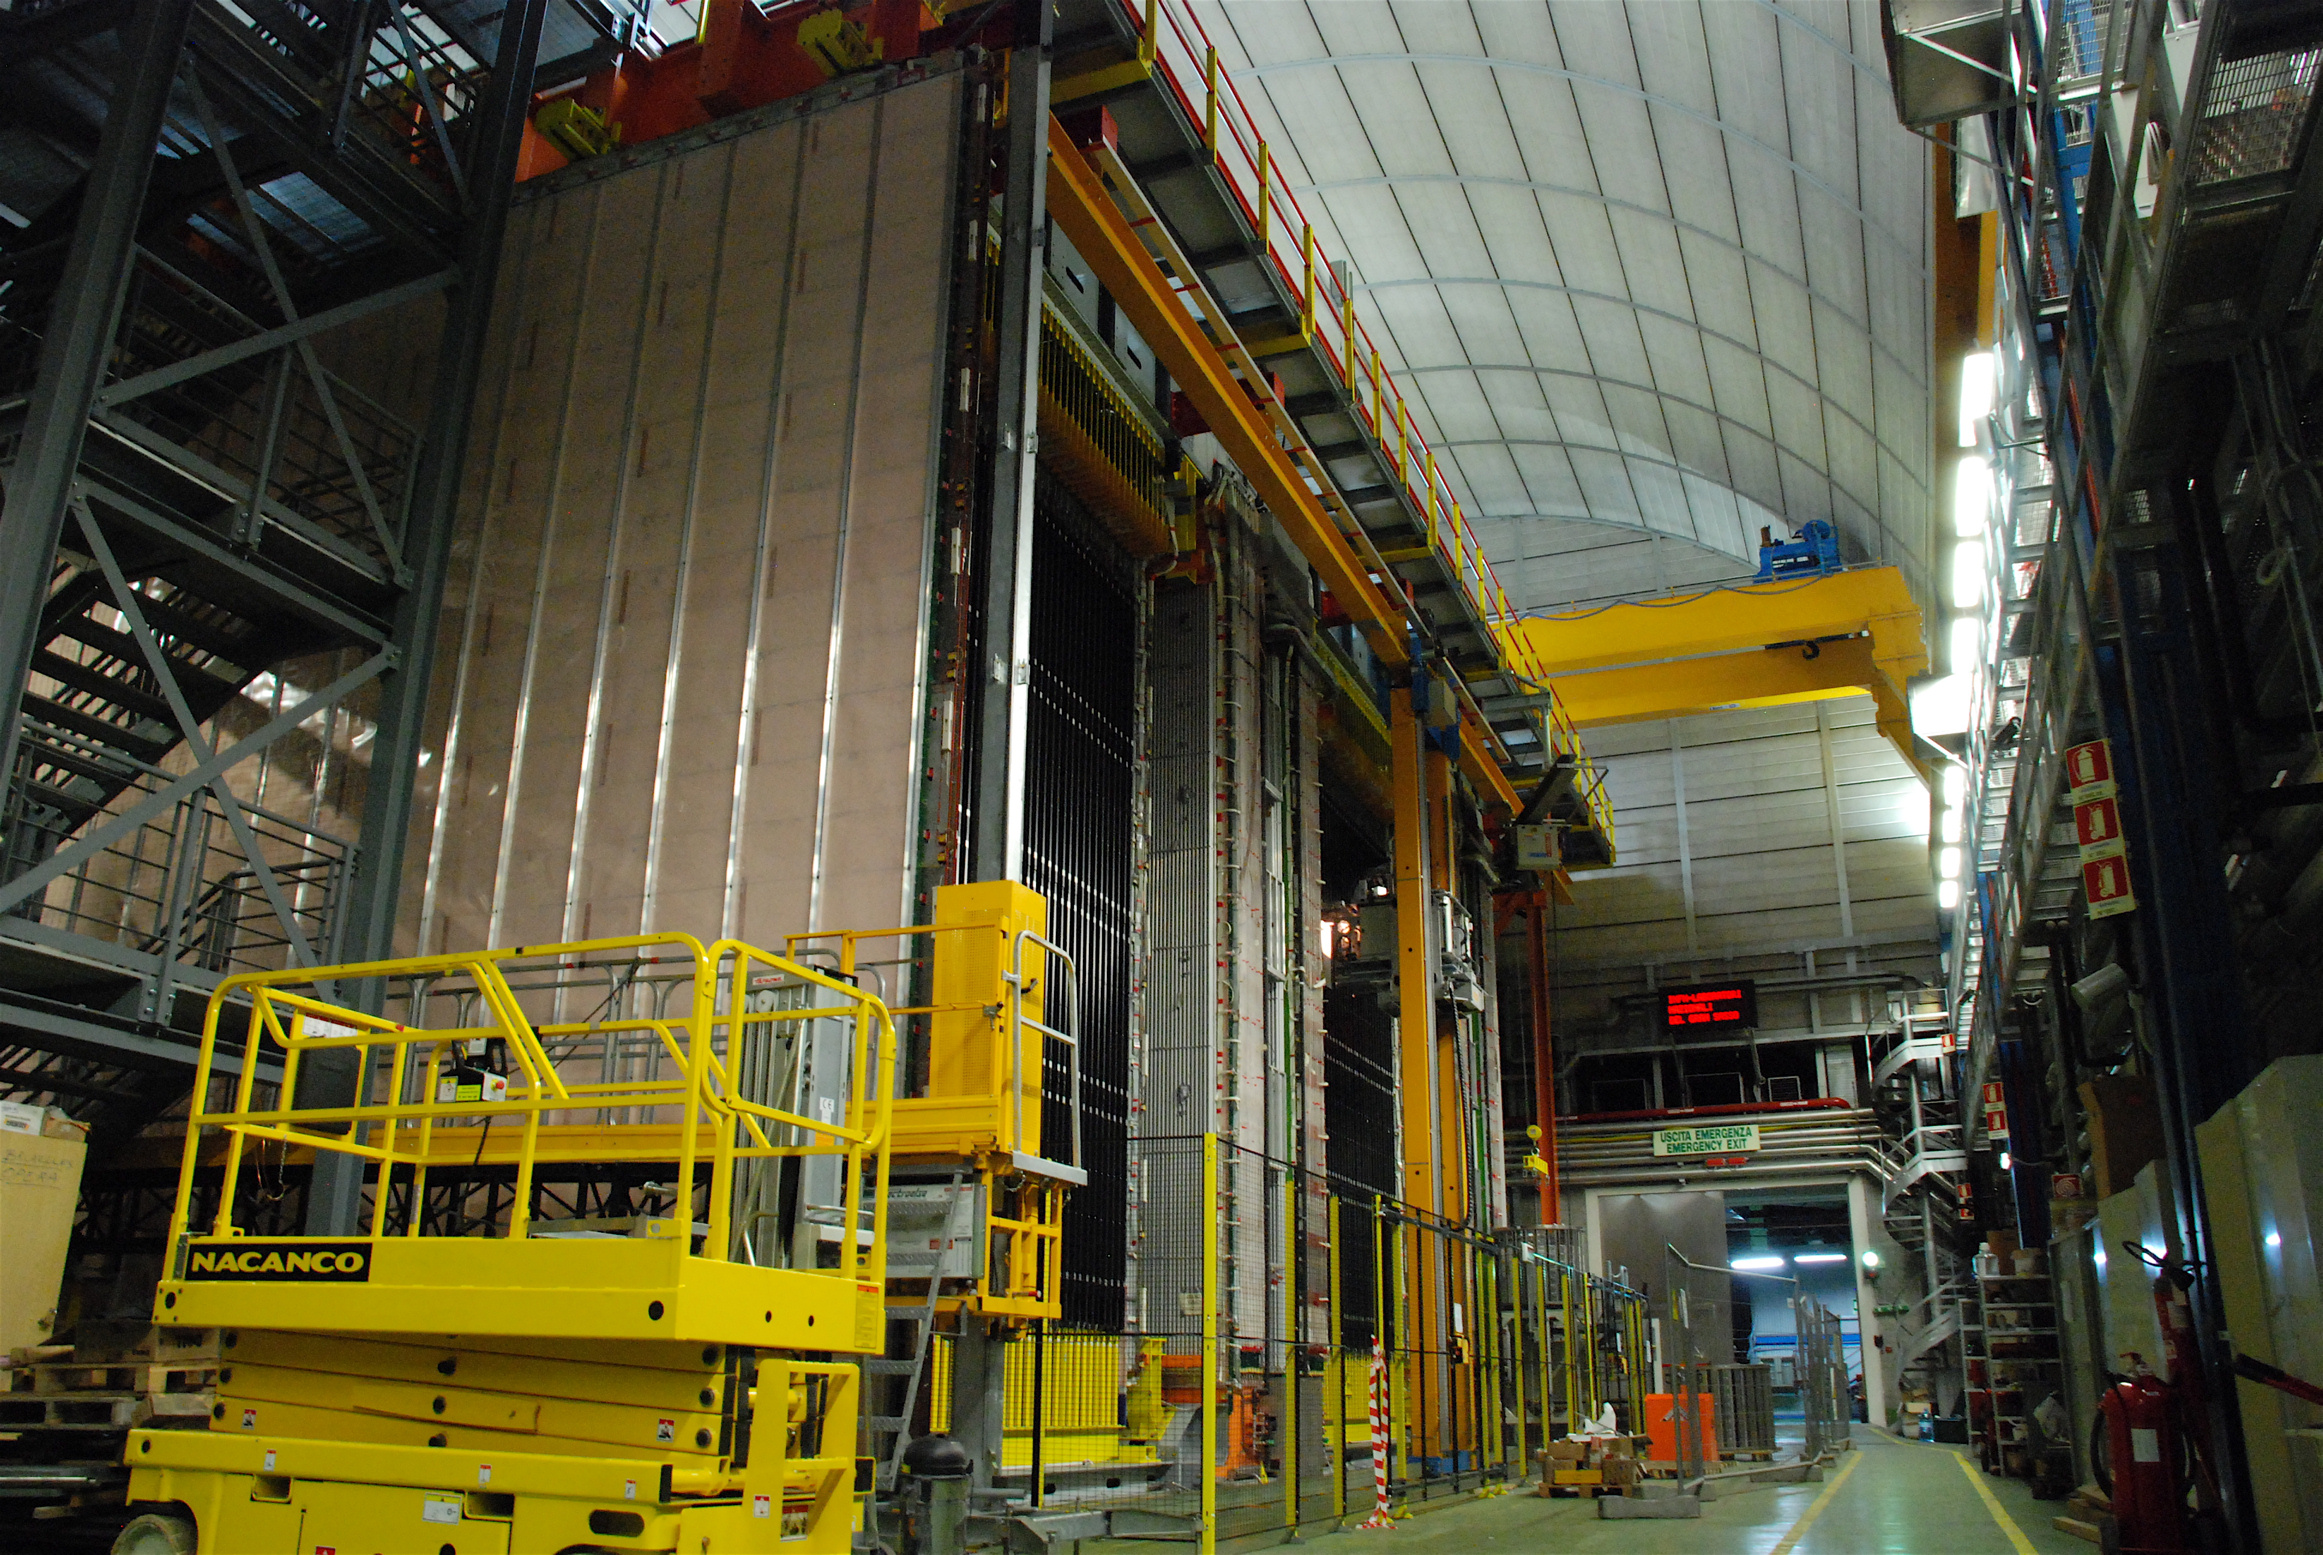
\includegraphics[width=\marginparwidth]{GLA/OPERA.jpg}
	\captionof{figure}{Photo du détecteur OPERA.}
	\label{opera}
}
\begin{figure}[h!]
	\centering
	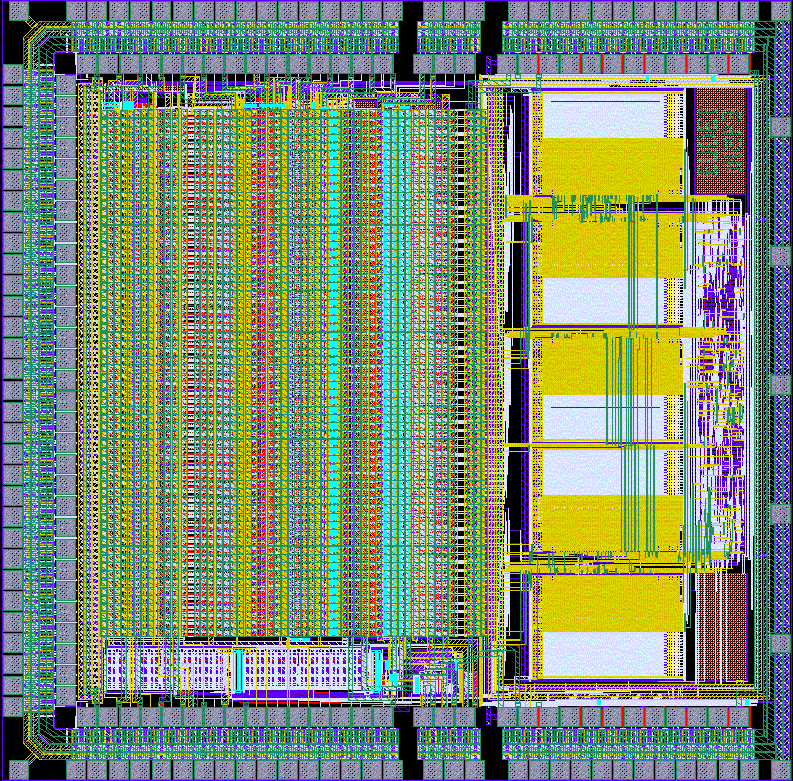
\includegraphics[width=0.5\textwidth]{GLA/HARDROC.png}
	\captionof{figure}{Schéma électronique du HARDROC.}
	\label{hardroc}
\end{figure}
Le HARDROC repose sur une technologie de fonderie AMS SiGe 0.5$\mu m$. La puce est ensuite insérée dans un boitier d'épaisseur 1.4mm qui comporte 160 pattes dont 64 voies. Les puces sont directement incorporées sur le PCB du détecteur appellée Active Sensor Unit (ASU), chaque HARDROC étant connecté à 64 bandes ou carreaux de cuivre sensitifs (strip et pads respectivement) selon le PCB. Dans le cas des pads, la connection des pattes et des carreaux des cuivre ont été étudiés afin d'éviter la diaphonie entre les pattes.
Le schéma simplifié du HARDROC est donné par la figure \ref{scheme}. La partie digitale de la puce est commune aux 64 voies, alors que chacune possède sa partie analogique :
\begin{figure}[h!]
	\centering
	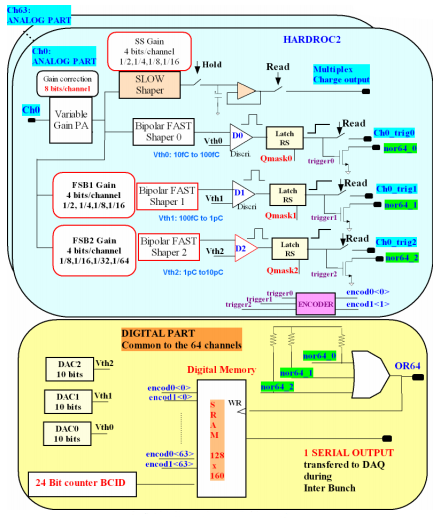
\includegraphics[width=0.8\textwidth]{GLA/scheme.png}
	\captionof{figure}{Schéma simplifié du HARDROC.}
	\label{scheme}
\end{figure}

Chaque voie d'entré est composée :
\begin{itemize}[label=$\bullet$]
	\item Un préamplificateur de basse impédance fonctionnant en mode convoyeur de courant dont le gain est ajustable de 0 à 1.99.
	\item Trois traitements de mise en forme rapide à gain réglable en parallèles (FSBs) (Fast Shaper). Ils sont suivis d'un discriminateur de tension qui une fois déclenché, active une bascule (pour la sauvegarde de l'information).
	\item Un traitement de mise en forme lent (Slow Shapper) qui permet le multiplexage du signal de sortie du préamplificateur et la lecture de la charge d'entrée. Ce traitement est surtout utilisé pour le débogage de la puce.
	\item Un encodeur pour coder le signal des bascules sur deux bits.
\end{itemize}

Les $3\times 64$ discriminateurs sont lus toutes les 200ns. Les trois seuils des discriminateurs peuvent être ajustés grâce à trois convertisseurs digital-analogiques (DAC) codés sur 10bits. Ce réglage affecte l'ensemble des 64 voies de la puce.

\subsubsection{Le préamplificateur}
L'entrée des cellules actives sont reliée aux pattes "in\_pa" d'un préamplificateur de type "Super Base Commune" (cf.fig\ref{preampli}), ce qui permet de diminuer l'impédance d'entrée (50-100 ohms) et donc d'éviter la diaphonie (\textit{cross-talk}). L'impédance d'entrée est donnée par la formule suivante :

\begin{equation}
Z_{in}=\frac{R_0+1/g_{m2}}{1+g_{m1}R_c}
\end{equation}
où $g_{m1}$ et $g_{m2}$ sont les transconductances des transistors $Q1$ et $Q2$ 

\begin{figure}[h!]
	\centering
	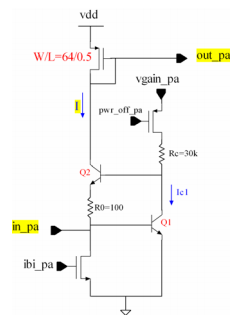
\includegraphics[width=0.5\textwidth]{GLA/preampli.png}
	\captionof{figure}{Schéma du préamplificateur.}
	\label{preampli}
\end{figure}

\subsubsection{Miroir de courant à 8 bits}
Le courant en sortie du préamplificateur est ensuite copié par huit miroirs de courant de gains respectifs 1/128, 1/64, 1/32, 1/16, 1/8, 1/4, 1/2 et 1 (cf.fig \ref{miror}). La sortie est la somme des courants des mirroirs activés. Les huit miroir sont activables séparément grâce à un mot de 8 bits appellé contrôl de gain. La plage d'amplification varie donc de 0 à 1.992. La précision de ce gain est estimé à 1.5\%. 

\begin{figure}[h!]
	\centering
	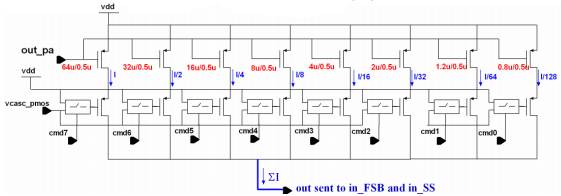
\includegraphics[width=0.8\textwidth]{GLA/miror.png}
	\captionof{figure}{Schéma du miroir de courant à 8 bits.}
	\label{mirror}
\end{figure}

\subsubsection{Les trois traitements de mise en forme rapide (FSB)}
En sortie du miroir à 8bits le signal passe dans trois circuit de traitement de mise en forme placée en parallèle. Ils consistent en un filtrage des signaux fournit en entrée afin d'éviter les perturbations dans le signal en sortie du préamplificateur ainsi que d'augmenter le rapport signal sur bruit. FSB1, FSB2 (cf.fig\ref{fsb1}) contrairement à FSB0 (cf.fig\ref{fsb0}) possèdent un système de 4 miroirs de courant afin de réduire le gain en entrée et ainsi augmenter la gamme dynamique. Le filtre FB0 est dédié aux charges d'entrée allant de 10fC à quelques centaines de fC, FSB1 qui posséde 4 miroir permet de traiter des signaux allant de 100fC à plus de 1pC; quant à FSB2 il permet de traiter des signaux de 1pC à 30pC.
\begin{figure}[h!]
	\centering
	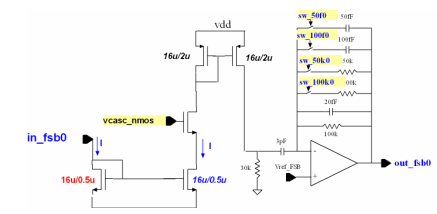
\includegraphics[width=0.8\textwidth]{GLA/FSB0.png}
	\captionof{figure}{Schéma de FSB0.}
	\label{fsb0}
\end{figure}
\begin{figure}[h!]
	\centering
	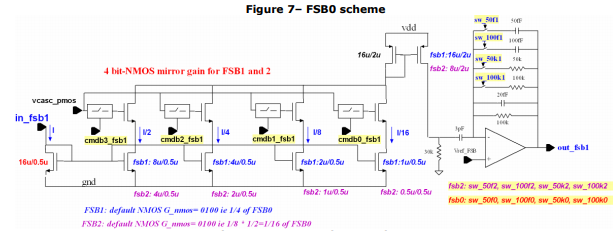
\includegraphics[width=0.8\textwidth]{GLA/FSB1.png}
	\captionof{figure}{Schéma de FSB1/2.}
	\label{fsb1}
\end{figure}
Il est possible d'activer des résistance et des condensateur dans le boucle de contre réaction du filtre (cf.fig\ref{fsb1},(cf.fig\ref{fsb0})), tout comme les gain des FSB, ils sont réglable par des mots de envoyé lors de la configuration des puces au début d'un run (slow control). Une étude poussée à été réalisé lors des test pour le SDHCAL et nous avons garder les valeurs trouvée comme les plus adaptées pour le gain des miroirs ainsi que pour la configuration de la boucle de contre-réaction.

La figure \ref{signal} montre la forme du signal en sortie des filtres FSB pour trois injections de charges différentes.
\begin{figure}[h!]
	\centering
	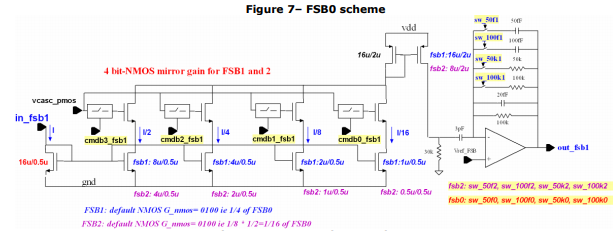
\includegraphics[width=0.8\textwidth]{GLA/FSB1.png}
	\captionof{figure}{Forme du signal en sortie des FSB pour des injections de charges de 100fC (bleu) , 1pC (vert) et 10pC (rouge). FSB0 à pour gain 1, FSB1 1/4 et FSB2 1/8}
	\label{signal}
\end{figure}

\subsubsection{Distriminateurs et bascules}
Chaque sortie de FSB est connectée à un discriminateur. Les seuils des discriminateurs est globale au 64 voies de la puce et sont réglable grâce à trois convertisseur digital-analogique (DAC) de 10 bits (de 0 à 1023). Il est donc possible de régler le seuil de manier à déclencher le discriminateur pour une charge donnée déposée sur les cellules actives du détecteur.

Les facteurs de conversion, qui permettent de passer de la valeur du DAC à la valeur du seuil sur la charge induite sur une cellule active, ont été déterminé à l'aide d'injections de charges. Un condensateur de 2 pF est activable par slow-control à cette effet, et permet d'injecter une charge donnée sur les 64 canaux du HARDROC. Pour chaque valeur de charge injectée, la valeur du seuil de basculement correspondant à une efficacité de détection de 50\% a été mesurée \cite{kieffer:tel-00751999}. Les courbes de ces valeurs de basculement pour chaque canaux en fonction de la charge injectée sont ensuite obtenues, pour chaque seuil. En soustrayant les piédestaux ont obtient les courbes suivantes :

\begin{figure}[ht!]
	\centering
	\subfloat[Seuil de basculement pour DAC0]{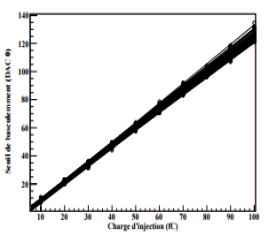
\includegraphics[width=.30\linewidth]{GLA/seuil1.png}}
	\hfill
	\subfloat[Seuil de basculement pour DAC1]{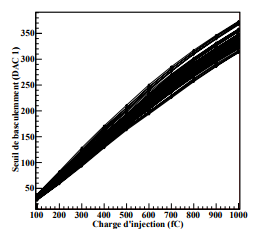
\includegraphics[width=.30\linewidth]{GLA/seuil2.png}}
	\hfill
	\subfloat[Seuil de basculement pour DAC2]{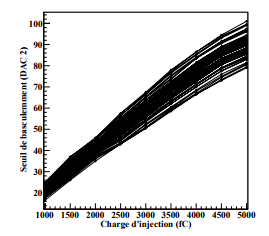
\includegraphics[width=.30\linewidth]{GLA/seuil3.png}}
	\caption{Seuil de basculement pour seuils (DAC0, DAC1, DAC2), en fonction de la charge injectée, pour 64 canaux d'un HARDROC. La valeur du piédestal a été soustraite.}
	\label{seuils}
\end{figure}

L'ajustement linéaire des courbes \ref{seuils} permet d'obtenir la valeur du seuil en fonction de la valeur de DAC pour chaque seuil :
\begin{equation}
Seuil_{i}=\frac{DAC_{i}-p_{i}}{\lambda_{i}} [pC]
\end{equation}
où $\lambda_{i}$ est le coefficient directeur de la droite obtenue après ajustement linéaire et $p_{i}$ est la valeur du piédestal. Les valeurs de ces paramètres pour chaque seuil sont donnés dans le tableaux suivant :
\begin{table}[H]
	\centering
\begin{tabular}{|O|O|O|N}
	\hline 
	Seuil & $\lambda$ & Piédestal \\ 
	\hline 
	0& 700 & 90 \\ 
	\hline 
	1& 80 & 98 \\ 
	\hline 
	2& 16.3 & 98 \\ 
	\hline 
\end{tabular} 
	\captionof{table}{Valeur des paramètres $\lambda$ et piédestaux pour les trois seuils.}
\end{table}
Les courbes \ref{seuils} n'étant pas linéaire sur toute la plage, nous nous avons veillé à ne pas dépasser la zone non linéaire lors de nos test en faisceau.

Chaque discriminateur est relié à une bascule de type RS qui, dés lors que le discriminateur correspondant est déclenché et le signal autorisant l'acquisiton est à l'état haut, passe à l'état haut. Lors du coup d'horloge suivant, tout les 200ns, les bascules sont lues et remise à zéro. Les trois valeurs des bascules correspondant à une cellule active sont ensuite envoyé dans un encodeur qui code ces informations sur deux bits selon le tableau \ref{tg}.
\begin{table}[H]
	\centering
	\begin{tabular}{|O|O|O|O|N}
		\hline 
		Seuil0  & Seuil1 & Seuil2 &Sortie \\ 
		\hline 
		0  & 0 & 0 & 00 \\ 
		\hline 
		1  & 0 & 0 & 01 \\
		\hline 
		1 & 1 & 0 & 10 \\
		\hline
		1  & 1 & 1 &11 \\
		\hline
	\end{tabular} 
	\captionof{table}{Encodage des seuils sur 2 bits.}
	\label{tabb}
\end{table}
Il est également possible de masquer une cellule active bruyantes en configurant la puce grâce de telle manière que la bascule soit à l'état bas en permanence. Ce réglage peut se faire grâce à des bits de masque envoyer lors du slow control.

\subsubsection{Le registre de contrôle lent (slow control)}
Afin de configurer le HARDROC, une patte d'entrée est utilisée. Une ligne d'horloge est mise en marche et à chaque front montant , les informations sont propagée dans le registre à décalage présent dans le HARDROC. 872 fronts d'horloge sont nécessaires afin de régler le HARDROC ( valeurs des seuils, gain des préamplificateurs, gains des FSB, masques etc...). Une fois toutes les informations envoyées, il suffit d'arreter l'horloge. La dernière bascule du registre est connecté à une patte qui permet à la fois de chainer les HARDROC et ainsi les configurer en série, mais aussi de vérifié que les bascules sont dans le bon état. Pour cela il suffit de redémarrer l'horloge et de comparer le mots binaire récupéré en sortie et le mots envoyé en entrée.

\subsubsection{La mémoire du HARDROC}
A chaque coup d'horloge, lorsque la puce est en phase d'acquisition, un OU logique est réalisé entre les bascules des 64 voies de la puce. Si l'une d'elle est à l'état haut, la mémoir digitale (Digital Memory) (cf.fig\ref{scheme}) reçoit un signal pour enregistrer l'événement. La valeur de l'horloge de l'événement, appellée Bunch Crossing ID (BCID) ainsi que le numéro d'identifiaction de l'ASIC ainsi que la valeur de tous les encodeur de la puce seront enregistrée. 

La mémoire du HARDROC permet de stocker 128 événement de 160bits (cf.tab \ref{bits}). Une fois sa mémoire pleine, un signal de saturation est émit sur une patte dédiée.
\begin{table}[H]
	\centering
	\begin{tabular}{|O|O|N}
		\hline 
		Contenu d'un événement (valeur autorisée) & Taille (octets) \\ 
		\hline 
		Header : Identifiant de l'ASIC (0-255)  & 1 \\ 
		\hline 
		BCID : Compteur d'horloge (0-16777215) & 3 \\
		\hline 
		États des canaux 48 à 63  & 4 \\
		\hline
		États des canaux 32 à 47  & 4 \\
		\hline
		États des canaux 16 à 31  & 4 \\
		\hline
		États des canaux 0 à 15  & 4 \\
		\hline
	\end{tabular} 
	\captionof{table}{Contenu d'un événement et taille en octet.}
	\label{bits}
\end{table}
 
\subsection{L'acquisition des données}
Le HARDROC à été conçu pour être chaîné, afin de piloter de nombreuses puces avec un nombres réduits de lignes communes. L'exemple du slow control montre l'intêret de ce chainage. Afin de gérer plusieurs HARDROC, une carte électronique composée d'un Field-Programmable Gate Array (FPGA), appellée Digital InterFace (DIF) (cf.fig\ref{DIF}) à été développé en collaboration avec le Laboratoire d'Annecy de Physique des Particules (LAPP). Cet carte possède un controleur USB utilisée pour le rappatriment des données, l'envoit des informations du slow control, d'un port HDMI dont le protocole permet la synchronisation des horloges et de connecter la DIF à une carte de contrôle. Elle dispose également de plusieurs entrées/sorties LEMO qui peuvent utilisée entre autres pour injecter un signal de déclenchement externe ainsi que de remonter un signal "busy".

\begin{figure}[h!]
	\centering
	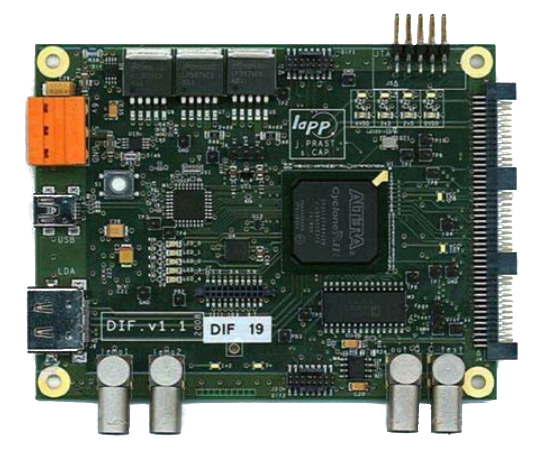
\includegraphics[width=0.6\textwidth]{GLA/DIF.png}
	\captionof{figure}{Photo d'une DIF.}
	\label{DIF}
\end{figure}

Pour commencer l'aquisition, la DIF envoie à tous les HARDROC un signal dit d'événement valide. Ceci à pour éffet de remettre à zéro leur compteur interne (BCID). Chaque événement correspondant à une cellule activé touchée est ensuite enregistré dans la mémoire du HARDROC connécté à cette cellule. Lorsque l'un d'un HARDROC à sa mémoire pleine, un signal de saturation est envoyé à la DIF par une ligne commune. On procéde alors à la lecture des mémoires des HARDROC (ReadOut). Chaque ASIC envoye le contenu de sa mémoire sur une ligne commune appellé ligne de donnée. Une ligne (Transmission ON) permet de prévenir la DIF qu'un des HARDROC procéde au transfert de ses données. Le fait de transférer les données en série améne à un temps mort maximum de
\begin{eqnarray}
n\times(128*160)bits\times 200ns= n*4.09ms
\end{eqnarray} 
où $n$ est le nombre de HARDROC. Une fois toutes les événements récoltés, les mémoires sont remises à zéro. Le diagramme temporelle \ref{temp} résume le cycle d'acquisition et de lecture décrit ci-dessus.

\begin{figure}[h!]
	\centering
	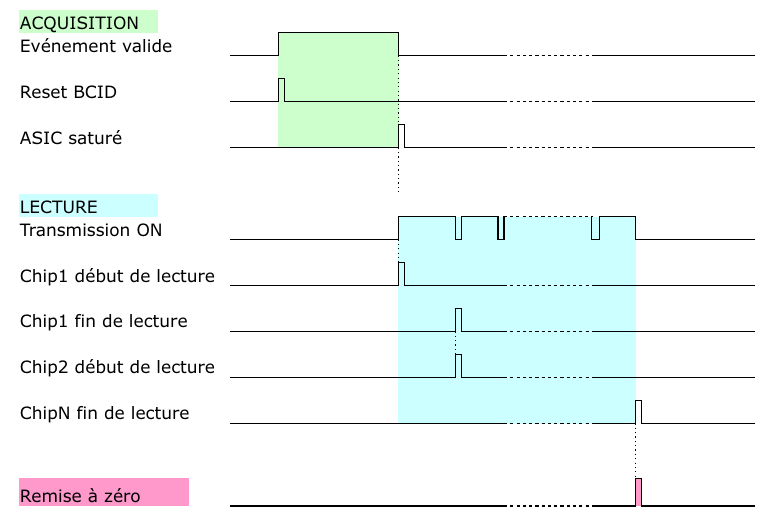
\includegraphics[width=0.6\textwidth]{GLA/cycle.png}
	\captionof{figure}{Diagramme temporelle du cycle d'acquisition et de lecture.}
	\label{temp}
\end{figure}
Afin de faciliter la reconstruction et l'analyse des données, des informations additionnelles sont ajoutées au flux de données des HARDROC par la DIF. À chaque ReadOut, les données des ASICS sont encapsulées par un header et un trailer ainsi que d'autres informations telles que des counteurs. Ces DIF sont reliées par l'intermédiaire de cable HDMI à une Synchronous Data Concentrator Card \footnote{Le nombre de chambre testées a toujours été inférieur à 9 ce qui permet de ce passer de DCC et de connecter directemen les DIF des chambres à la SDCC.} \cite{Baulieu:2015pfa} qui reçoit les busy et les RAMfull des DIF et envoye de manière synchrone l'horloge et les commandes. La carte SDCC est directement reliée par USB à l'ordinateur controllant la DAQ.

La chaine d'acqusisiton peu être résumé apr le schéma suivant : 
\begin{figure}[h!]
	\centering
	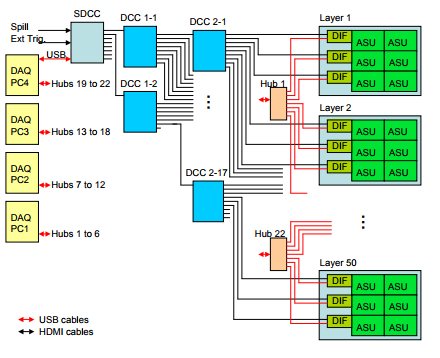
\includegraphics[width=0.6\textwidth]{GLA/chaine.png}
	\captionof{figure}{Architecture de la DAQ du SDHCAL. Dans notre cas le nombres d'ASU est d'un par layer (chambre) ainsi que d'une DIF par chambre. Le nombre de chambre étant dans notre cas inférieur à 9 l'utilisation des DCC est inutiles. }
\end{figure}

\subsection{Format de donnée LCIO}
La chaine d'acquisition et l'électronique ayant été conçus pour le détecteur ILD de ILC, les données sont sauvegarder dans le format de données Linear Collider I/O (LCIO)\cite{2003physics6114G}. Ce format repose sur un modèle d'événement générique  dans lequel les données sont organisées en collections. Chaque collection contient une liste d'object dont la structure est adaptée à l'information à stocker ainsi qu'une liste de paramètre. À chaque début d'acquisiton un fichier LCIO est créeé et les événements sont stocker dans un LCEvent contenant une collection d'objets de type LCGenericObject ("RU XDAQ") qui contiennent les données brutes de chaque DIF enregistrées sous forme d'entiers.

Ces fichiers peuvent ensuite être lus et analysés en créant des algorithme qui sont implémenté sous forme de processeur codé en c++ et utilisé par framework Modular Analysis \& Reconstruction for the LINear collider (MARLIN) \cite{Gaede:2006pj}. Chaque processeur analyses les données dans les LCEvent e permettent de créer de nouvelles collections qui sont ajouté à l'événement ou sont inséré dans les LCEvents d'un nouveau fichier. MARLIN permet de définir les processeur et l'ordre dans lequel les lancer à l'éxécution sans recompilation. Pour cela il utilise un fichier xml de configuration appellé "steering file". Ils est également possible de définir dans ce fichiers les paramètres nécessaire au processeur.

\section{Programme d'analyse pour les chambres à élecronique HARDROC}
L'un des travaux de notre thèse a été de se familiariser avec ce framework et de programmer des processeur afin d'analyser les données en provenance des détecteurs. 

\subsection{Les processeurs MARLIN}
Trois processeurs permettent de structurer les données afin d'en tirer les caractéristiques des détecteurs présentées précédemment :

\begin{itemize}[label=$\bullet$]
	\item Le processeur Streamout permet de mettre en forme les données brutes et de passer des LCGenericObject en une collection de RawColorimeterHit qui correspondent à des cellules touchées. Ces objects contiennent le numeros de la voies touchées du HARDROC (Channel\_Id), le numéro de l'HARDROC touché (ASIC\_Id) ainsi que le numéro de la DIF s'occupant de cet HARDROC (DIF\_Id).
	\item Le processeur Trivent permet de passer du triplet (Channel\_Id,ASIC\_Id,DIF\_Id) à la position local dans la chambre (I,J,K=numero de la chambre) . La position des chambres (DIFS) dans l'espace est contenu dans un fichier Extensible Markup Language (XML) qui est un paramètre du steering file de MARLIN, CE QUI PERMET des positions locale dans une chambre à la position réelle dans l'espace de la cellule touchée (X,Y,Z). Trivent permet aussi de présélectionner les candidats muons. En effet, les données récoltés correspondent à tous les hits collectés jusqu'à ce qu'un Hardroc soit plein. Les données colléctées inclues non seuelement des hits venant de muons mais aussi des hits de bruits etc. Pour sélectionner les candidats muons clusterisation en temps est réalisé. Les coups d'horloge (BCID) qui présentent plus de $M_{hit}=3$ sont sélectionné. Pour chaque coup d'horloge sélectionné, les hits appartenant à des coups d'horloge contenu dans une fenêtre de $\pm t_{fen}=\pm3$ sont combiné pour construire un candidat muon. Si deux candidats sont proches et leur fenêtres se chevauchent ils ne sont pas pris en compte afin de ne pas ajouté plusieurs fois les hits dans plusieurs candidats muons. Chaque hits sélectionné pour un même candidat muons appartiennent à une meme collection et à un même événement.
	\item Le processeur Analysis utilise ces candidats muons et effectue une sélection pus fine des candidats muons. Premièrement les évènement contenant un trop gros nombre de hits dans une chambres sont rejectés. Afin d'estimé l'éfficacité d'une chambre, les barycentres des hits des autres chambres sont utilisées afin de créer un candidat trace. Pour cela une minimisation par $\chi^2$ est utilisé. Les $\chi^2$ réduit $\chi^2/ndf$ sont données par :
	\begin{equation}
	\chi_{xz}^2/ndf=\sum_i^{Nplate-1}(x(z_{i})-x(z_{i})_{ba}) \quad \chi_{yz}^2/ndf=\sum_i^{Nplate-1}(y(z_{i})-y(z_{i})_{ba})
	\end{equation}
	où $x(z_{i})_{ba})$ et $y(z_{i})_{ba}$ sont les coordonnées du barycentre des hits dans la chambre $i$ et :
\begin{equation}
\begin{cases}
\strut x(z_i)=az_i+b\\
y(z_i)=cz_i+d
\end{cases}
\end{equation}
est l'équation paramétrique d'une droite dans l'espace avec 4 paramètres $a,b,c,d$. La minimisation est effectué grâce au paquet MINUIT \cite{James:2004xla} contenu dans le framework ROOT \cite{BRUN199781}.
Si la droite traverse la chambre étudié et si des hits sont situé à dans une region de $\pm 3 cellules*\pm 3 cellules$, $\pm 3 strips$ du point d'impact, la chambre est considéré efficace pour cette événement. Le nombre de hits dans cette région est utilisé comme estimateur de la multiplicité du détecteur.
\end{itemize}

Le fait d'avoir conçu les processeur de telle manière que la géométrie ne soit connue que dans un fichier XML possède de nombreux avantages. Cela permet notamment de pouvoir changer facilement une DIF ou une chambre du détecteur sans avoir à recompiler les processeurs, de garder une trace des géométries utilisées sous forme lisible et claire. Cela à également permis de faire fonctionner ces processeur sur une simulation du prototype du SDHCAL afin de vérifier que ces processeur donnés la bonne éfficacité alors que ni le nombres de chambres (48 pour le SDHCAL), ni le nombres d'ASU et de DIF par chambre (6 et 3 resectivement ) sont identiques à nos détecteurs placés en test en faisceaux.

\subsubsection{Test des processeurs par une simulation du SDHCAL}
Le test des processeur utilise une simulation du SDHCAL basé sur GEANT4\cite{AGOSTINELLI2003250} qui calcule les sections efficaces lors de la propagation des particules dans le détecteur. Le champ électrique entre les deux électrodes de verre des GRPC ne sont pas simulé. En revanche, les avalanches sont modélisées par un algorithme appellé SimDigital qui est en fait un processeur MARLIN disponible dans le paque MarlinReco \cite{2007Prama} de ILCSoft. Cet algorithme s'occupe également de la répartition de la charge sur les carreaux de cuivre. Une description détaillé de cet algorithme ainsi que de son paramétrage est donné dans \cite{steen:tel-01282680}.

L'algorithme utilise les segments de GEANT4 créés par les particules incidentes chargés. Il arrive cependant, que plusieurs segments soient créés par GEANT4 pour une même particule incidentes dans la même couche de gaz. Ces segments pourraient chacun produire une avalanche. Afin d'éviter que cela n'arrive, les segments sont reliés entre eux.

 À chaque volume de gaz correspondant à une cellule de lecture $C_{0}$, la longueur des segments contenus dans ce volume est calculé. Les segment de taille inférieur à 1$\mu m$ sont supprimé.
 
 Une carte d'efficacité pour chaque ASIC est ensuite appliqué afin de tenir compte des gaz CO2 eet SF6 dont les effets ne sont pas pris en charge par GEANT4. Il est aussi possible de forcer les efficacité d'une chambre par ces cartes. Une chambre possédant une carte d'efficacité de 50\% aura donc 50\% que les segments passant par sa couche de gaz soient conservés.
 
 La charge induite par chaque segment est ensuite aléatoirement choisie en utilisant une distribution de Polya:
 \begin{eqnarray}
 P(q)=\left[\frac{q}{\bar{q}}(1+\theta)\right]^\theta\exp^{-\left[\frac{q}{\bar{q}}(1+\theta)\right]}
 \end{eqnarray}
 où $\bar{q}$ est la valeur moyenne en pC et $\theta$ une paramètre libre lié ç la largeur de la distribution. Afin de tenir compte de l'angle d'incidence, la charge induite est corrigée $Q_{corr}$.
 
 Lorsque deux avalanches sont très proches l'une de l'autre et se chevauchent, le signal induit n'est pas la somme des signaux de chaque avalanches. Pour simuler cette effet, lorsque deux segments sont situés à une distance inférieur à une valeur $d_{cut}$, seule le segment dont la charge induite est la plus élevée est gardé.
 
 La charge induite est ensuite répartie sur la cellule $C_0$ et sur les cellules voisines se trouvant à une distance inférieur à $r_{max}$ de $C_0$. Un rapport est alors calculé pour chaque cellule :
 \begin{equation}
 R_i=\frac{\int_{a_i}^{b_i}\int_{c_i}^{d_i}\sum_{j=0}^{n-1}\alpha_j\exp^{\frac{(x-x_0)^2+(y-y_0)^2}{2\sigma_j^2}}\dd x\dd y}{\int_{-r_{max}}^{+r_{max}}\int_{-r_{max}}^{+r_{max}}\sum_{j=0}^{n-1}\alpha_j\exp^{\frac{(x-x_0)^2+(y-y_0)^2}{2\sigma_j^2}}\dd x\dd y}
 \end{equation}
où $a_i$, $b_i$, $c_i$ et $d_i$ sont les positions des bords de la cellule $i$, $(x_0,y_0)$ sont les coordonnées du milieu du segment, $n$, $\alpha_j$ et $\sigma_j^2$ sont des paramètres libres. Ainsi $C_0$ est ses voisins se voit ajoutés une charge induite de $R_iQ_{corr}$.

Pour finir les seuils des cellules sont appliqués. Seuls les cellules possédant une charge supérieur au seuil seront considéré comme étant touchée et créent un hits.

Nous avons utilisé cette simulation en simulant le passage de muons de 100 GeV dans le prototype SDHCAL dont les cartes d'efficacités des 48 chambres ont été fixé successivement de 10\% à 100\% par pas de 10\%. La figure \ref{effisimul} montre les efficacités calculées par le processeur Analysis pour les 48 chambres du SDHCAL et les 10 cartes d'efficacité.

\begin{figure}[h!]
	\centering
	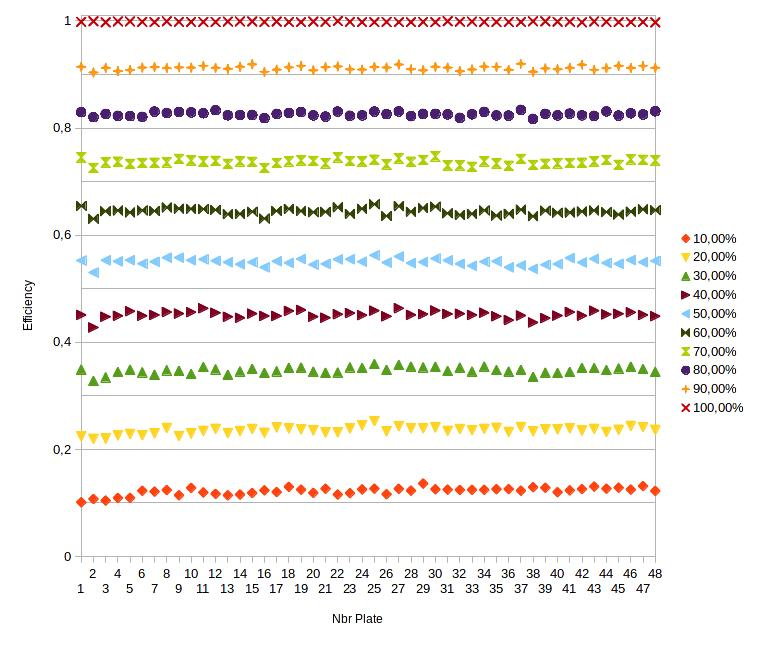
\includegraphics[width=0.9\textwidth]{GLA/effisimul.jpg}
	\captionof{figure}{Efficacité trouvé par le processeur Analysis pour les 48 chambres du SDHCAL en utilisant la simulation SimDigital. Les particules incidentes sont des muons de 100GeV et chaque couleur représente une carte d'efficacité fixé lors de la simulation.}
	\label{effisimul}
\end{figure}

Cette figure montre bien que l'on arrive a retrouvé l'efficacité fixé dans par les cartes d'efficacités de la simulation. Une divergence semble apparaitre et augmenter jusqu'à 50\% puis diminuer. Elle est au maximum de 5\%. Elle peut s'expliquer par la manière dont les traces sont regroupés. Tous les résultats présentés dans cette thèse qui ont rapport avec des chambres instrumenté avec des HARDROC ont été réalisé avec ces processeurs.

\section{Tests en faisceaux}
De nombreux tests en faisceaux ont été réalisés lors de cette thèse, notamment afin de vérifier et de compléter les résultats obtenus lors d'un test en faisceau à DESY en Allemagne en Janvier 2012.
\subsection{Test en faisceau à DESY}
Un test en faisceau à DESY \cite{Haddad:2012fx} a été réalisé afin de vérifier les caractéristiques des verres de basses résistivité produit par l'université de Tsinbghua. Des chambres en verre de basse résistivité de 30*30cm2 (GRPC) (cf.fig\ref{chambre}) instrumenté par une électronique composé de HARDROC et de cellule de lecture en forme de pads (cf.fig\ref{cellule}) ont été soumis à un faisceau intense et continu d'électron d'énergie allant jusqu'à 6GeV couvrant une surface de quelques cm2. Le flux d'électrons est au maximum de 35KHz. Le mélange de gaz est composé de 93\% de TFE(C2F4), 5\% de CO2 et 2\% de SF6 (mélange ILC).
\begin{figure}[h!]
	\centering
	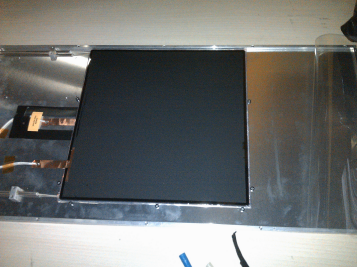
\includegraphics[width=0.5\textwidth]{GLA/chambre.png}
	\captionof{figure}{Photo d'une GRPC composée de verre de basse résistivité ($\sim 10^10 \Omega .cm$).}
	\label{chambre}
\end{figure}
\begin{figure}[h!]
	\centering
	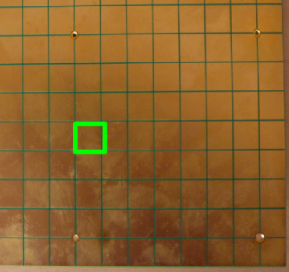
\includegraphics[width=0.3\textwidth]{GLA/cellules.png}
	\captionof{figure}{Cellules de lecture de taille 1cm*1cm, une cellule est encadré en vert}
	\label{cellule}
\end{figure}

Ce test en faisceau à montré que les verre de basse résistivité pouvait supporté un flux de particule de 9kHz/cm tout en gardant une efficacité proche de 90\% (cf.fig\ref{effiDesy}). Le point de fonctionnement à été estimé à 7.2kV donnant une efficacité de 95\% est une multiplicité de 1.4, pour un seuil de 50fC. 
\begin{figure}[h!]
	\centering
	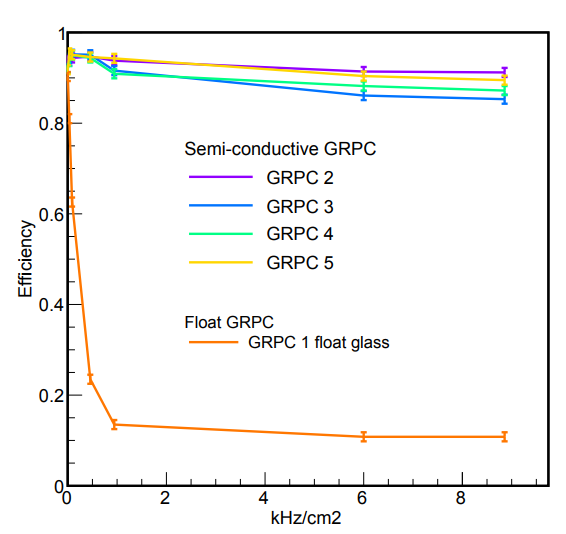
\includegraphics[width=0.9\textwidth]{GLA/effiDesy.png}
	\captionof{figure}{Efficacité en fonction du flux de particule pour différents GRPC. La ligne orange correspond à une chambre composé de verre "Standard" dit \textit{Float Glass} de resistivité de l'ordre de $10^13 \Omega.cm$. Les autres courbes correspondent à des chambres composées de verre de basse résistivité. }
	\label{effiDesy}
\end{figure}

Alors que dés 1kHz, les chambres de verre standard voient leur efficacités chuter autour de 20\%, les chambres construites avec des électrodes en verre de basse résistivité continues à être efficaces même après 9kHz. Leurs efficacité décroit très lentement en fonction du flux de particules.

